\section{Methodology}

% このセクションの構成
まずプロンプトの生成方法、軸があって、そこにペルソナをいれる。軸とペルソナは今回の政治ドメインでは、XXXを使います。

最後にテクニカル貢献を述べる


\label{sec:methodology}

\begin{figure*}[htbp]
    \centering
    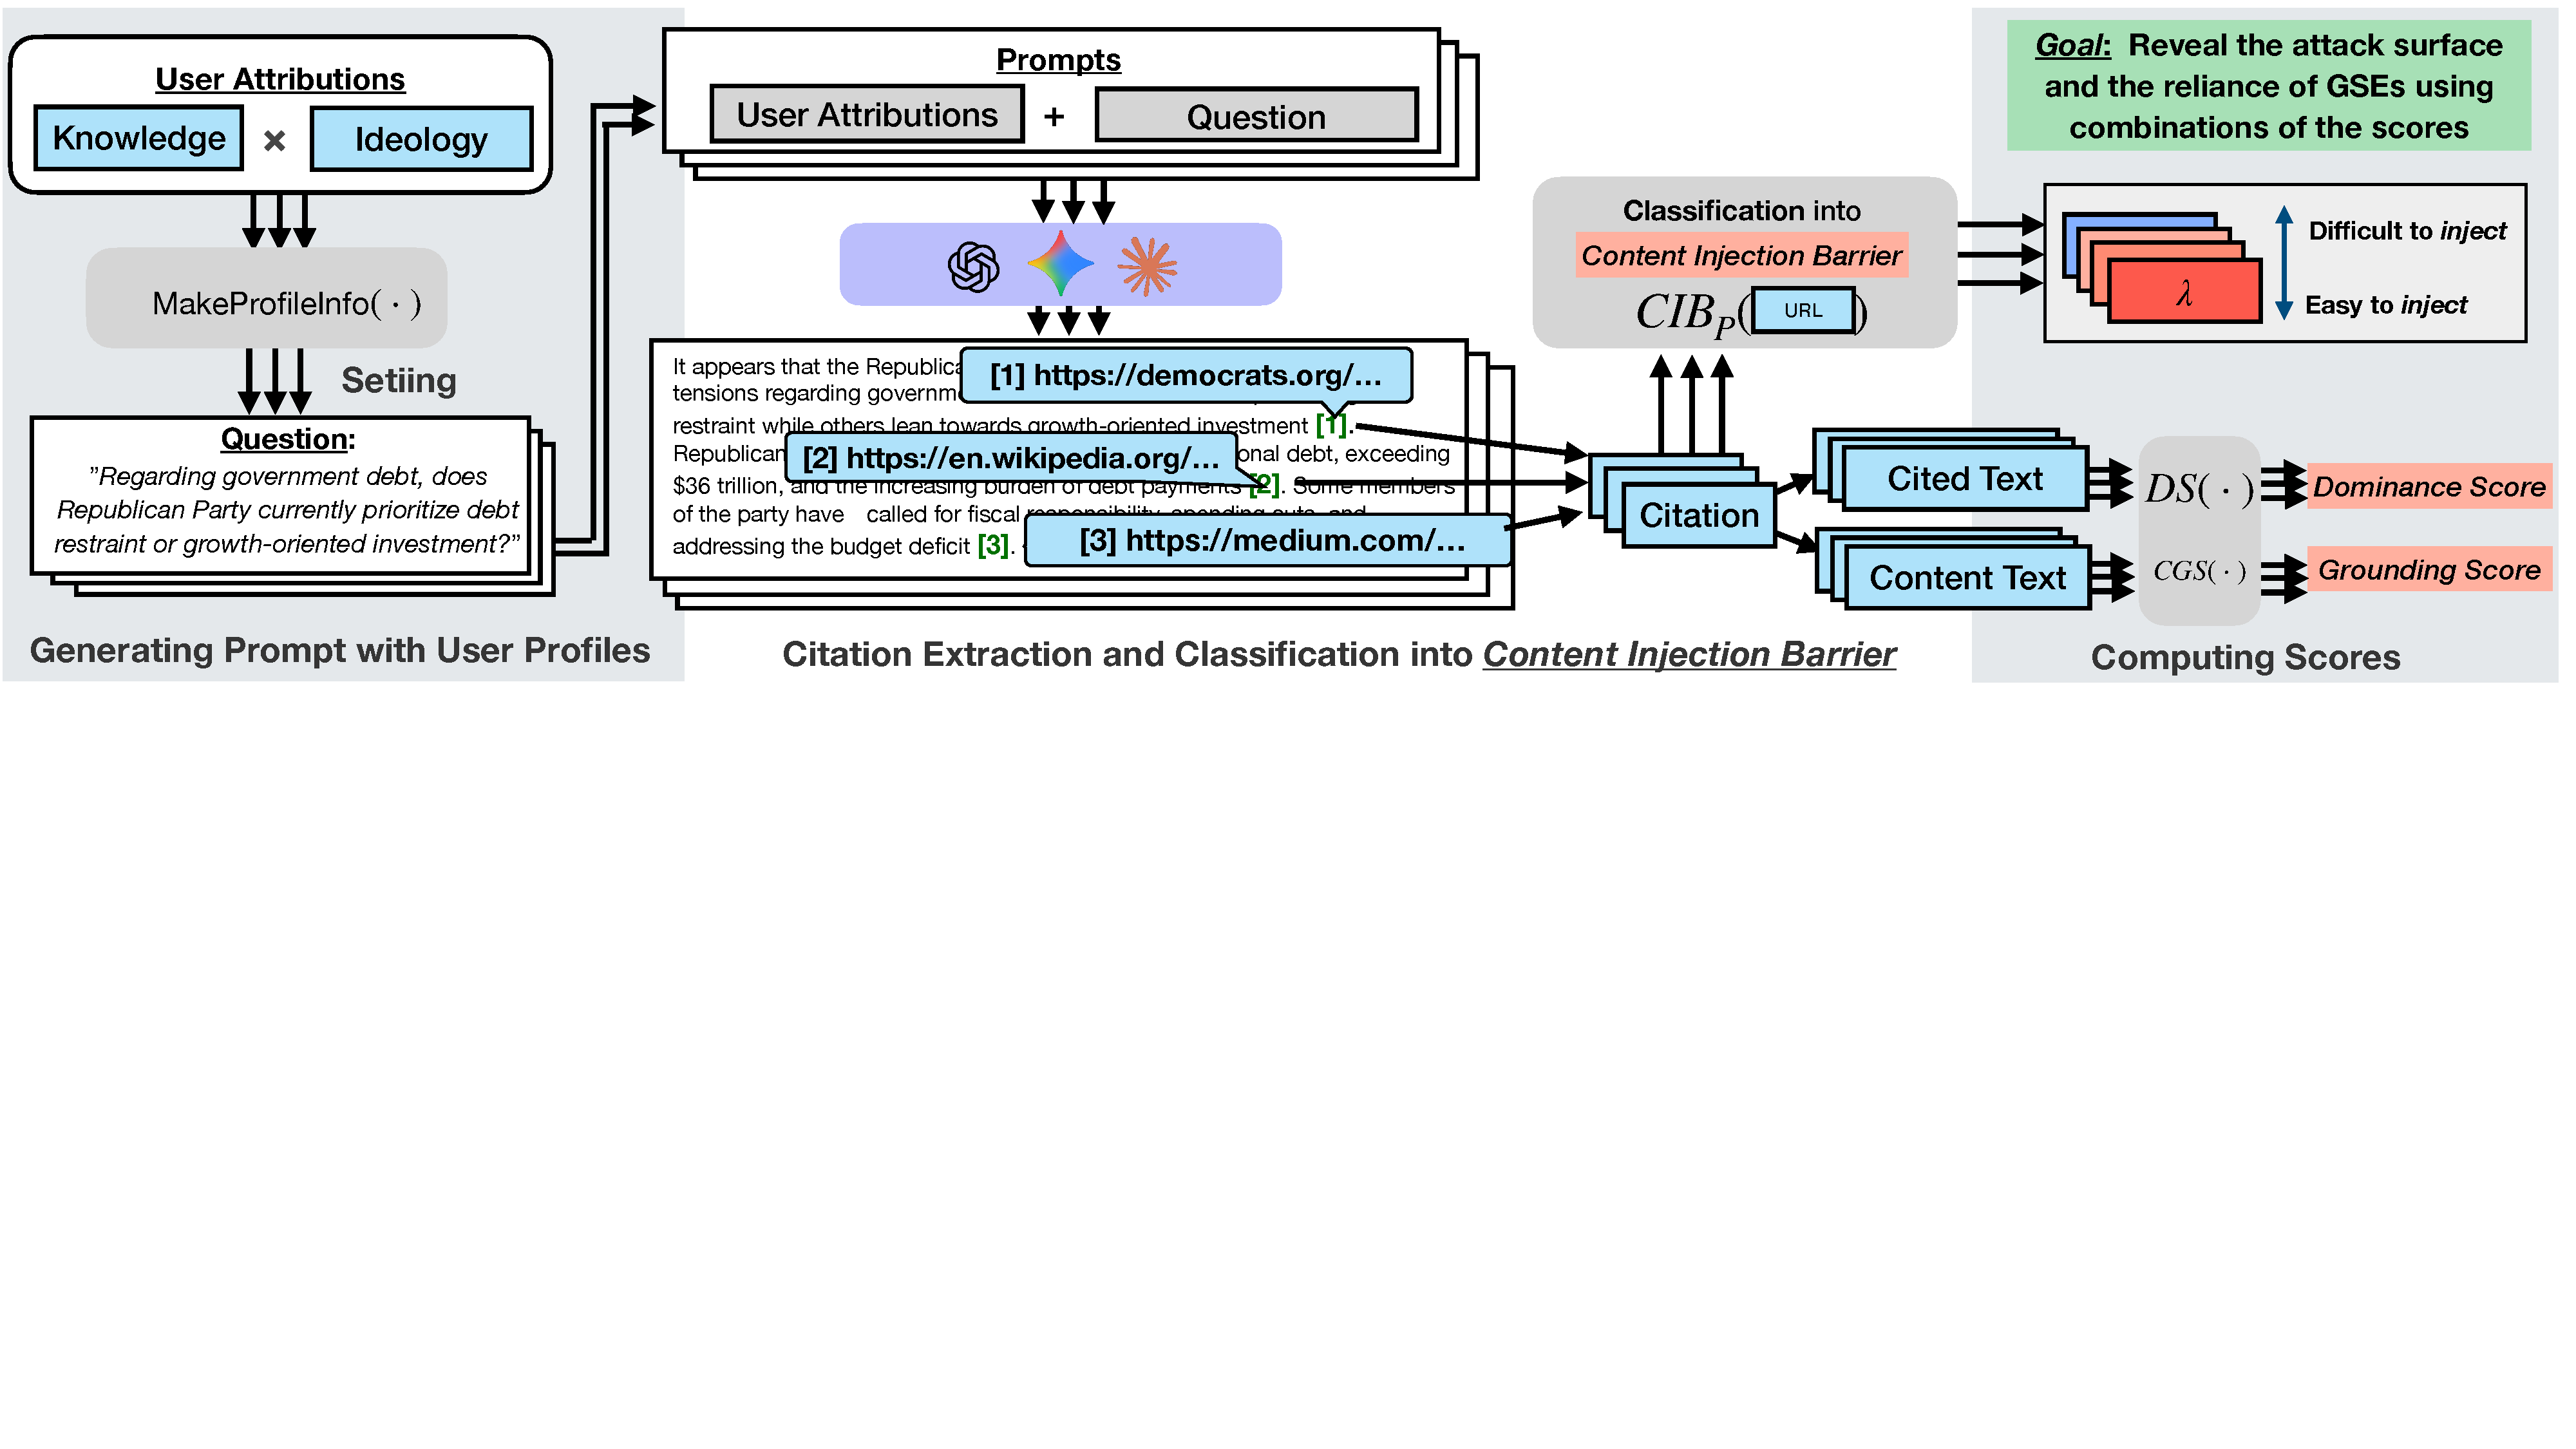
\includegraphics[width=1.0\textwidth]{figs/overview.pdf}
    \caption{Our research goals and methodology. We aim to characterize the attack surface of GESs to poisoning attacks by analyzing the publisher attributes of citations as \emph{content-injection barriers} in generated answers.}
    \label{fig:overview}
\end{figure*}

% To reveal which publisher attributes GESs preferentially cite, we propose a method to classify the publisher attributes of web content cited by GESs.
We introduce novel evaluation criteria that focus on the publisher attributes of citations in answers to characterize the attack surface of GESs to poisoning attacks.

Our study aims to reveal two types of bias and define research questions:
\emph{R-1}: Which publisher's content GESs preferentially cite and reveal bias of citation selection from the perspective of publishers?
\emph{R-2}: How publisher's content has the power to influence the content of generated answers faithfully?
By providing evaluation criteria that can answer these questions, we enable users and communities to assess whether vulnerable behaviors under PoisonedRAG attacks exist in GESs according to the nature and target of information retrieval, thereby contributing to the monitoring and maintenance of the safety of GESs.
% We discuss the relationship between the nature of information retrieval targets and the threat of PoisonedRAG attacks on GESs as a ideal citation balance in Section~\ref{sec:discussion}.

% 権威性を基にしたクラスタリングとGESの特性をこのカテゴリを元に行うことで、攻撃者はどのような権威性を持つWeb出版者からコンテンツを発信しなければGESsにおける回答をゆがめられないのか、、
To reveal these biases, we propose a component to classify the publisher attributes of citations in answers.
In this component, we define the difficulty of publishing content on the web with specific publisher attributes as the \emph{content-injection barrier} and categorize publishers of citations based on these barriers into low-, medium-, and high-barrier categories.
% ここから下は最後時間があるときまで文言考えたい、なんか腑に落ちない。
Using this barrier, we can reveal which level of publisher authority attackers must achieve to successfully inject malicious content and influence GES answers.
By clustering citations based on content-injection barriers and analyzing GES behavior by the barriers, we can assess the practical difficulty and threat of poisoning attacks.

% To derive this barrier, we classify publisher attributes to publisher categories and then derive the content-injection barrier based the publisher categories.
% Second, we propose two evaluation criteria: (1) distribution of content-injection barriers in answers and (2) distribution of semantic consistency by content-injection barriers.
Finally, we introduce a citation reflection component to reveal the bias of citation reflection from the perspective of publisher attributes.
This component quantifies the influence of each content of citations on answer generation by using similarity-based methods.
We show the overview of our goals and proposed methodology in Figure~\ref{fig:overview}.
% We then use these components to answer the research questions \emph{R-1} and \emph{R-2} in experiments in Section~\ref{sec:experiment}.

\subsection{Citation Classification}
\label{subsec:citation_classification}
The first component classifies citations in answers into content-injection barriers.
We introduce a classifier \( \psi_{\mathcal{P}}(c) \) that assigns each citation \( c \) to an appropriate \emph{content-injection barrier} for each target political party \( \mathcal{P} \).
In our experiments in Section~\ref{sec:experiment}, we target the questions in the political domain; thus, in explanation, we denote \( \mathcal{P} \) as the target political party.
We divide the classification into three components: primary information identification, secondary information category classification, and content-injection barrier classification.
We perform multi-stage classification to ensure interpretability of the clustering results.
Because content-injection barriers are abstract high-level categories, we ensure the validity and interpretability of this categorization by first classifying publishers into primary and secondary information sources, then categorizing secondary sources into fine-grained publisher categories, and finally deriving content-injection barriers from these categories.

\textbf{Primary Information Identification.}
We identify primary information sources that are directly relevant to specific domains.
First, we define the target domain set \( \mathcal{D}_{\mathcal{P}} \) (e.g., $\mathcal{P}$ is the U.S. Democratic Party, \( \mathcal{D}_{\mathcal{P}} = \{\text{democrats.org, democrats.gov, democrats.io}\} \)).
Let \( d_c = \text{domain}(c) \) be a function extracting the domain from each citation \( c \in C \).
We check whether \( \mathcal{D}_{\mathcal{P}} \) includes \( d_c \).
When \( d_c \) is included in \( \mathcal{D}_{\mathcal{P}} \), we classify the citation as a primary information source.
Here, \( \mu_{\mathcal{P}}(c) \) outputs 1 if \( d_c \) is included in \( \mathcal{D}_{\mathcal{P}} \) and \(\bot\) otherwise.

\textbf{Secondary Information Category Classification.}
We categorize secondary information into fine-grained publisher categories, which serve as intermediate categories for calculating content-injection barriers.
We prepare publisher category set \\ \( \Pi = \{\pi_1, \pi_2, \cdots, \pi_p\} \). 
Here, \( \pi(c) \) maps citation \( c \) to category \( \pi; i \in \{1, 2, \cdots, p\} \).
In our experiments in Section~\ref{sec:experiment}, we use labels such as ``Party'', ``Media'', ``Platform'', ``Owned'', ``Academia'', and ``Non-media-industry''.

To build the function \( \pi(c) \), we adopt a hybrid strategy combining automatic category classification using LLM-as-a-Judge~\cite{survey-llm-as-a-judge-arxiv24,judging-llm-as-a-judge-with-mt-bench-and-chatbot-arena-arxiv23} and manual category classification.
We prepare two GES models (ideally two models from different providers such as GPT and Gemini with web search mode enabled) and use them to identify publishers from domains and WHOIS information.
Combining multiple GES models can reduce potential biases of single GES models and increase classifier accuracy~\cite{judging-llm-as-a-judge-with-mt-bench-and-chatbot-arena-arxiv23}.
When classification results from the two GES models agree, we adopt that result directly; when they disagree, we perform manual classification.
In our experiments, the authors make the final determination based on company information from the website and domain registration data.
We employ zero-shot classification~\cite{radford2019language} following Kostina et al.~\cite{kostina2025largelanguagemodelstext}, who demonstrate high performance without training examples.
For each citation \( c \in C \), the prompt receives two inputs: \( \text{url}(c) \) extracts the complete URL indicating the publisher's domain and path, and \( \text{whois}(c) \) retrieves domain registration data including ownership and organizational information.
We provide the complete classification prompt template and the domain-to-category mapping table used in our experiments in our repository~\cite{QL_CIKM_RERO}.
% Finally, we obtain the set of citations classified into each category \( \lambda_i \) as \( C^{\lambda_{i}} = \{c \in C \mid \lambda(c) = \lambda_i\}; i \in \{1, 2, \cdots, p\} \).

Finally, we derive content-injection barriers from these categories.
Here, \( \lambda_{\mathcal{P}}(\pi) \) maps publisher category \( \pi \) to content-injection barrier \( \Lambda = \{\lambda_1, \lambda_2, \cdots, \lambda_q\} \). 
We define five content-injection barriers \( \Lambda \): \emph{Primary Sources}, \emph{Opponent Sources}, \emph{Low-Barrier Sources}, \emph{Medium-Barrier Sources}, and \emph{High-Barrier Sources}.
\emph{Primary Sources} are domains owned by the party referenced in the question. If \( \mu_{\mathcal{P}}(c) = 1 \), then \( c \) is classified as a primary information source.
\emph{Opponent Sources} are domains operated by rival parties. If \( \mu_{\mathcal{P}}(c) = \bot \) and \( \pi(c) \) is ``Party'' in our experiment, then \( c \) is classified as an opponent information source.
\emph{Low-Barrier Sources} are domains where users or owners can freely publish or edit content (``Platform'' and ``Owned'' in our experiments).
\emph{Medium-Barrier Sources} are domains owned by organizations or companies with editorial processes where journalism bias or interests may appear (``Media'' and ``Non-media-industry'' in our experiments).
\emph{High-Barrier Sources} are domains where authors are required to remain neutral and objective and manipulation is difficult (``Academia'' and ``Government'' in our experiments).


\subsection{Citation Reflection}
\label{subsec:citation_reflection}
The second component measures the semantic consistency of citations and answers and calculates the citation reflection power for each citation content.
We introduce a classifier \( \tau(c, r) \) that classifies each citation \( c \) and answer \( r \) into an appropriate \emph{similarity band} \( T = \{\tau_1, \tau_2, \cdots, \tau_b\} \).
We decompose the measurement into two steps:

\textbf{Decomposing Answers and Citations into Sets of Sentences.}
First, we decompose answer \( r \) into sentences \( S = \{l_1, l_2, \ldots, l_k\} \) and each citation \( c_i \in C \) into sentences \( S_{c_i} = \{s_{i,1}, s_{i,2}, \ldots, s_{i,n_i}\} \).
Because some sentences of answer \( r \) have citation labels attached and the semantics of each answer sentence is independent, we need to decompose answer \( r \) into sentences to evaluate similarity accurately.
% To decompose answer \( r \) and citation \( c_i \) into sentences, we introduce a sentence splitting function \( \text{SentenceSplit}(x) \) which decomposes text \( x \) into sentences.

\textbf{Similarity Measurement.}
We measure textual and semantic similarity between each answer sentence \( \{l_1, l_2, \ldots, l_k\} \) and each citation sentence \( S_{c_i} = \{s_{i,1}, s_{i,2}, \ldots, s_{i,n_i}\} \) for each citation \( c_i \in C \).
To measure similarity between two sentences, we introduce the calculation of similarity function \( \text{sim}(x, y) \) between two sentences \( x \) and \( y \).
The function \( \text{sim}(x, y) \) returns a similarity score between the two sentences \( x \) and \( y \) as a value in the range of \( -1 \) to \( 1 \).
Here, a similarity value closer to \(-1\) indicates lower semantic similarity, whereas a value closer to \(1\) indicates higher semantic similarity.
To calculate the similarity, we employ Sentence-BERT~\cite{sentence-bert-arxiv19}, which converts each sentence into dense embedding vectors and computes their semantic similarity through cosine similarity.
In our experiments in Section~\ref{sec:experiment}, we utilize the pre-trained Sentence-BERT model ``stsb-xlm-r-multilingual''~\cite{sentence-bert-arxiv19}, which has been trained on multilingual semantic textual similarity tasks.

\textbf{Maximum Similarity Identification.}
GESs often use only some sentences within long citation texts to generate particular answer sentences, thus we identify the maximum similarity between the answer sentence set \( S \) and citation \( c_i \) to reveal the reflection power of a citation in answers.
Finding the maximum similarity identifies the most relevant part of the citation text to the answer content.
In detail, we calculate the maximum similarity as \( \text{sim}_{\text{max}}(S, c_i) = \max_{j \in \{1,\ldots,k\}, m \in \{1,\ldots,n_i\}} \text{sim}(l_j \in S, s_{i,m} \in S_{c_i}) \).
In calculating this maximum similarity, we compute the similarity between each answer sentence \( l_j \in S \) and all sentences \( s_{i,m} \) within citation \( c_i \) and adopt the highest similarity value across all combinations.

Finally, we categorize the maximum similarity scores \( \text{sim}_{\text{max}}(S, c_i) \) into three \emph{similarity bands} \( T \) to reveal the reflection power of a citation in answers.
We introduce a $\gamma(\text{sim}_{\text{max}}(S, c_i))$ function that maps the maximum similarity score to the similarity band:
\emph{High} similarity (scores in \([0.9, 1.0]\)) indicates strong semantic alignment between answer and citation sentences, suggesting direct reflection of the citation source in the answer.
\emph{Mid} similarity (scores in \([0.8, 0.9)\)) represents moderate semantic overlap, indicating partial citation contribution.
\emph{Low} similarity (scores in \([-1.0, 0.8)\)) reflects weak semantic connection, suggesting minimal reflection of the citation source in the answer.
We employ these thresholds because \(0.8\) has been used as a threshold for detecting paraphrased sentences~\cite{kabir2024banglaembed} and \(0.9\) for classifying similar sentences~\cite{tumre2025improved} in prior studies.

% \textbf{Citation reflection power classification.}
% After obtaining maximum similarity scores \( \text{sim}_{\text{max}}(S, c_i) \) for each citation \( c_i \in C \), we categorize each citation using the above content-injection barrier classifier \( \Lambda(\cdot) \).
% This categorization allows us to examine how different content-injection barriers are reflected faithfully in answers at varying similarity levels.
